
\documentclass[border=10pt]{standalone}
\usepackage{pgfplots}
\pgfplotsset{compat=1.18}
\begin{document}
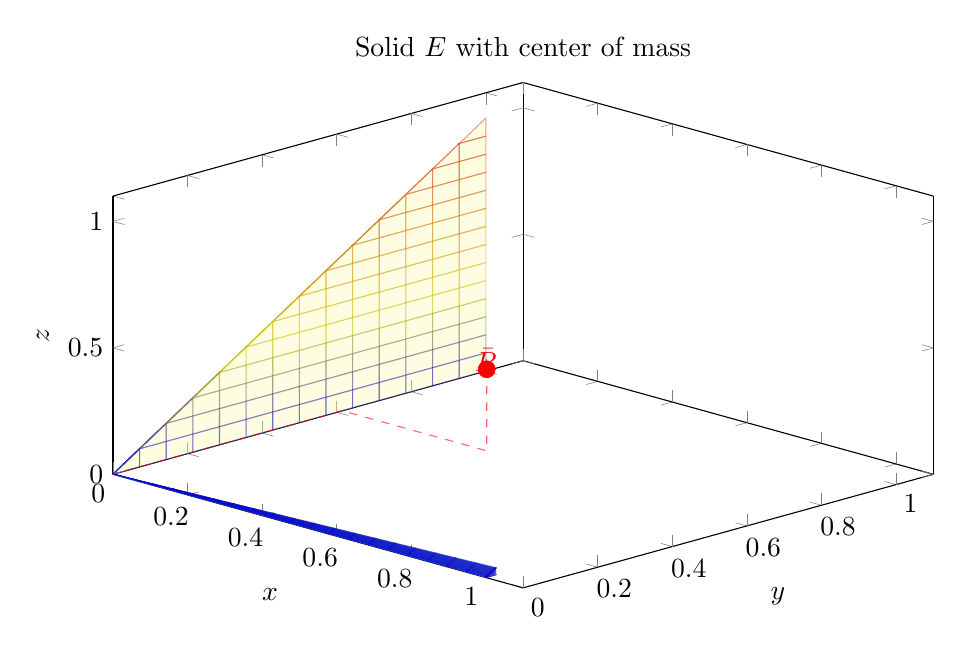
\begin{tikzpicture}
\begin{axis}[
    width=12cm, height=8cm,
    view={45}{30},
    xmin=0, xmax=1.1, ymin=0, ymax=1.1, zmin=0, zmax=1.1,
    xlabel={$x$}, ylabel={$y$}, zlabel={$z$},
    title={Solid $E$ with center of mass},
]
% Top surface z = y over quarter disk, parametrize by r and theta
\addplot3[
    surf, mesh/ordering=y varies,
    domain=0:1, y domain=0:1.5708,
    samples=20, samples y=20,
    opacity=0.6, fill=cyan!50, draw=black,
] ({x*cos(y)}, {x*sin(y)}, {x*sin(y)});

% Cylinder side r=1, 0<=theta<=pi/2, 0<=z<=sin(theta)
\addplot3[
    surf, mesh/ordering=y varies,
    domain=0:1, y domain=0:1.5708,
    samples=20, samples y=20,
    opacity=0.4, fill=blue!20, draw=black,
] ({cos(y)}, {sin(y)}, {min(x, sin(y))});

% Plane x=0 face: y in [0,1], z in [0,y]
\addplot3[
    surf,
    domain=0:1, y domain=0:1,
    samples=15, samples y=15,
    opacity=0.4, fill=yellow!30, draw=black,
] (0, {x}, {min(x,y)});

% Center of mass
\addplot3[only marks, mark=*, mark size=3pt, red] coordinates {
    (0.3874, 0.6150, 0.3223)
};
% Drop lines
\addplot3[dashed, red, opacity=0.6] coordinates {
    (0.3874, 0.6150, 0.3223) (0.3874, 0.6150, 0)
    (0.3874, 0.6150, 0) (0, 0.6150, 0)
    (0, 0.6150, 0) (0, 0, 0)
};
\node[red] at (axis cs:0.5, 0.5, 0.45) {$\bar{P}$};
\end{axis}
\end{tikzpicture}
\end{document}
